\ifdefined\BuildingFromMainFile
\else
   \documentclass[../main.tex]{subfiles}
   \begin{document}
\fi


\graphicspath{{figure/}{../figure/}}

\clearpage
\onehalfspacing

\linespread{1.25}
\setlength{\parskip}{\baselineskip}

\normalsize


This thesis is the first to investigate the utility of genome graph-based approaches in the cattle genome. Thereby, this thesis offers a novel paradigm in the analysis of livestock genomes through accounting for genetic diversity in all subsequent genomic analyses. The graph-based approaches introduced here facilitate variation-aware genetic analyses in which that individual DNA sequences are compared to a set of haplotypes observed in the population rather than to the linear reference genome, which is highly biased. Graph-based approaches have never been investigated in species with gigabases of genome other than human. Within this thesis, I constructed the first genome graphs in any livestock species and performed different analyses to investigate the utility of genome graph-based approaches (Table \ref{tab51:comp}).  

Using three different variation-aware genome graphs, this thesis has demonstrated  that genome graphs outperform linear genomes across a suite of genomic analyses. Chapter 3 and 4 showed that graph-based reference structures enable improvements in mapping rate and resolve misalignments to the linear genome. These mapping improvements facilitate accurate and unbiased genotyping. Chapter 3 showed that genotyping based on the graph-based alignment yielded a more balanced support of both reference and alternate allele. These findings suggest enormous potentials of genome graphs for analyses which are sensitive to allelic dosage, such as allele-specific expression studies that can leverage complete variations in an unbiased way. More importantly, multi-assembly graphs constructed in Chapter 4 readily reveal the more complete bovine pangenome, including abundant biologically-relevant sequences which are missing in the current ARS-UCD1.2 \emph{Bos taurus} reference genome. Genome analyses are currently blind to the variations in these missing segments. Thus, the pangenome graph-based approach introduced in Chapter 5 makes this so far unused source of variations amenable for genomic analysis. Chapter 4 also provides an example how these hitherto neglected sequences enable a better biological understanding of the molecular underpinnings of phenotypic variation. 

\section{The application of graph genomes in cattle population}

\subsection*{The feasibility of graph-based genomic methods on the cattle genome}

Chapter 2 investigated the utility of region-specific graphs for the genotyping of polymorphic sites in the cattle genome. This type of variation-aware graph is augmented with variants discovered from an initial linear alignment of the same sequenced cohort. The workflow was established based on a modified version of the \emph{Graphtyper} 


\begin{landscape}
   \thispagestyle{plain}
   \begin{table}
      \centering
      \footnotesize
      \caption[Comparison of the genome graph implementations]{\textbf{Comparison of the three genome-graph approaches implemented in this thesis}}
      \begin{tabular}{|l|l|l|l|} 
      \cline{2-4}
      \multicolumn{1}{l|}{~}                                                                              & \multicolumn{1}{c|}{\textbf{Chapter 2}}                                                                                                                                                                                                                                 & \multicolumn{1}{c|}{\textbf{Chapter 3}}                                                                                                                                                                                   & \multicolumn{1}{c|}{\textbf{Chapter 4}}                                                                                                                                                                                                                            \\ 
      \hline
      \textbf{Graphs}                                                                                     & Local (region-specific) ~variation graphs                                                                                                                                                                                                                               & Whole-genome (full)variation graphs                                                                                                                                                                                       & Multi-assembly genome graphs                                                                                                                                                                                                                                       \\ 
      \hline
      \textbf{Graph constructor}                                                                          & \textit{Graphtyper}                                                                                                                                                                                                                                                     & \textit{vg toolkit}                                                                                                                                                                                                       & \textit{minigraph}                                                                                                                                                                                                                                                 \\ 
      \hline
      \begin{tabular}[c]{@{}l@{}}\textbf{Source of variations}\\\textbf{added to the graphs}\end{tabular} & \begin{tabular}[c]{@{}l@{}}Cohort-specific variants of\\49 Original Braunvieh\end{tabular}                                                                                                                                                                              & \begin{tabular}[c]{@{}l@{}}External (known) variants of \\288 cattle across four breeds\\(OBV, Brown Swiss, Fleckvieh, Holstein)\end{tabular}                                                                             & \begin{tabular}[c]{@{}l@{}}6 genome assemblies\\(OBV, UCD, Angus, Highland, Brahman, Yak)\end{tabular}                                                                                                                                                             \\ 
      \hline
      \textbf{Application of the graph}s                                                                  & \begin{tabular}{@{\labelitemi\hspace{\dimexpr\labelsep+0.5\tabcolsep}}l@{}}\begin{tabular}[c]{@{}l@{}}Refined genotyping \\from linear alignment\end{tabular}\end{tabular}                                                                                              & \begin{tabular}{@{\labelitemi\hspace{\dimexpr\labelsep+0.5\tabcolsep}}l@{}}Variant prioritization\\Genotyping from full-graph alignment\\Assessment of reference bias\end{tabular}                                        & \begin{tabular}{@{\labelitemi\hspace{\dimexpr\labelsep+0.5\tabcolsep}}l@{}}SV and non-reference sequences extraction\\Prediction of the novel genes\\Transcription potential of non-reference sequences\\Genetic variants in non-reference sequences\end{tabular}  \\ 
      \hline
      \textbf{Benefits}                                                                                   & \begin{tabular}{@{\labelitemi\hspace{\dimexpr\labelsep+0.5\tabcolsep}}l@{}}Computationally efficient\end{tabular}                                                                                                                                                       & \begin{tabular}{@{\labelitemi\hspace{\dimexpr\labelsep+0.5\tabcolsep}}l@{}}Incorporate known (external variations)\\Full-graph based alignment\\More extensive downstream tools~\\that can process the graph\end{tabular} & \begin{tabular}{@{\labelitemi\hspace{\dimexpr\labelsep+0.5\tabcolsep}}l@{}}\begin{tabular}[c]{@{}l@{}}Include large segments (structural variations) \\diverged between assemblies\end{tabular}\\Computationally efficient~\end{tabular}                           \\ 
      \hline
      \textbf{Limitations}                                                                                & \begin{tabular}{@{\labelitemi\hspace{\dimexpr\labelsep+0.5\tabcolsep}}l@{}}\begin{tabular}[c]{@{}l@{}}Need initial global read alignment~\\by a linear mapper\end{tabular}\\Region-specific graphs\\Limited by small variations~\\discovered in the cohort\end{tabular} & \begin{tabular}{@{\labelitemi\hspace{\dimexpr\labelsep+0.5\tabcolsep}}l@{}}Computationally expensive\\Limited by small variations\end{tabular}                                                                            & \begin{tabular}{@{\labelitemi\hspace{\dimexpr\labelsep+0.5\tabcolsep}}l@{}}Not including small variations\\\begin{tabular}[c]{@{}l@{}}Dependence of the graph backbone \\and order of assembly included\end{tabular}\\Limited downstream tools~\end{tabular}       \\
      \hline
      \end{tabular}
      \label{tab51:comp}
      \end{table}
\end{landscape}


software that was compatible with cattle chromosome complement. Even though, that the pipeline is not full graph-based, as it depends on variants discovered from linear alignments and global read placement by a linear mapper, this simple graph-based implementation exceeded the performance of the current-state-of-the-art linear mapping. Variant genotyping was highly accurate as indicated by multiple metrics including genotype concordance, non-reference sensitivity, non-reference discrepancy, and mendelian inconsistencies, suggesting that graph-based methods are readily applicable for genomic analyses of the cattle genome. 

\subsection*{Local graph genotyping is competitive with state-of-art linear-genome based methods}

The computational requirement (both memory and time) is lower for the \emph{Graphtyper}-based than the \emph{GATK}–based variant discovery, which is a best practice pipeline that also performs local read re-alignment. Therefore, the application of a region-specific graph-based method is competitive with the linear genome. In fact, the original \emph{Graphtyper} implementation in humans has been applied to genotype thousands of  human DNA samples demonstrating that it is applicable to genotype variants at the population scale \citep{eggertsson2017graphtyper,eggertsson2019graphtyper2}. However, it turned out that the graph-based method struggles with gaps and potential miss-assemblies that were numerous in the bovine UMD3.1 assembly. An additional analysis conducted in Chapter 2 provides evidence that these problems are mostly resolved when the updated cattle reference genome (ARS-UCD1.2) is used, likely because it is more complete and contiguous than UMD3.1 \citep{rice2020continuous}. Thus, this thesis suggests that graph-based methods will benefit from the current large influx of reference-quality assemblies across a wide-range of species. 

Chapter 2 further demonstrated that genotypes produced by graph-based analysis are compatible with current state-of-the-art downstream tools can directly make use of the output. First, the genotype likelihoods produced by Graphtyper may serve as input and benefit from Beagle imputation, even yield higher genotype concordance compared to imputation using genotypes from a linear-mapping based methods. Secondly, we discovered more than 17 million variants from 49 key ancestor animals of the Original Braunvieh cattle breed using Graphtyper and used these genotypes to assess genomic diversity \citep{bhati2020assessing}. 

\section{Variant prioritization to include in the graphs}

Instead of only using genetic variants from the same cohort, informative graphs may also be constructed using external variants. The study presented in Chapter 3 utilizes a catalogue of variants discovered from close to 300 cattle from four major European cattle breeds to build variation-aware graphs. This approach showed that graph-based analysis can leverage on a readily available variant database. 

It is well known that variant prioritization is crucial to construct informative graph genomes \citep{pritt2018forge,jain2021variant}. Chapter 3 showed that adding random unphased variants without any prioritization increases graph complexity without any benefits on read mapping accuracy. Chapter 3 demonstrated that variant prioritization based on allele frequency is most crucial to increase the read mapping accuracy. Adding more variants prioritized based on allele frequency increases the mapping accuracy. However, the addition of variants with frequencies between 0.01 to 0.1 did not further improve the accuracy. Thus, there seems to be an optimal number of included variants to create an informative graph genome. The addition of variants beyond this threshold will not lead to an additional gain in the accuracy. Our investigations revealed that this threshold is population-specific. For example, the negative impact of rare variants on mapping accuracy was more pronounced in the human than cattle population, possibly due to human datasets being more enriched  for low-frequency variants. 

Chapter 3 showed that pangenome graphs performed similar  to population (breeds) specific graphs. A similar finding has recently reported from a pan-human consensus reference \citep{kaminow2020virtue} suggesting the limit of including population-specific variations. This further suggests that building a unified cattle pangenome graph is possible and likely preferred over generating multiple population-specific graphs. Due to low effective population size, a common set of variants to be added to the pangenome can be detected from few key ancestor animals, which have been compiled for instance by the 1000 Bull Genomes Project \citep{hayes20191000}.  Chapter 3 shows that this observation holds for variation-aware graphs from four European cattle breeds. These breeds share more than 80\% of the variations. Yet, it remains to be investigated  if this graph is also applicable to genetically-diverged breeds. Possibly, a set of prioritized variants from genetically-diverged breeds can be added to the graph while  increasing the graph complexity is paid off with gaining informativeness. The pervasive introgression and admixture across \emph{Bos} species seem to indicate that this is a viable strategy \citep{wu2018pervasive}. Ideally the graph includes variants from all global breeds (including understudied breeds), which will provide insight into an unbiased picture of the cattle diversity. 

\section{Investigation of the inaccessible genetic variations with multi-assembly graphs}

\subsection*{Multi-assembly graph provides a platform to investigate complete genetic variations }

Beyond integrating small variations as in the Chapter 2 and 3, graph genomes provide a more powerful framework to investigate large variations between individuals \citep{eggertsson2019graphtyper2,chen2019paragraph,siren2020genotyping}. So far, there are only a few studies have attempted to characterize structural variations in the cattle genome \citep{liu2010analysis,bickhart2012copy,boussaha2015genome,chen2017detection,Hu2020}. However, large variations on overall affect longer genomic regions than small variations and have a more drastic effect on the gene functions \citep{chiang2017impact,scott2021structural}. Thus, the contribution of structural variations shape the cattle genome architecture is likely to be under-appreciated. For example, a SV study as a part of  1000 Bulls genome project \citep{chen2017detection} found an overrepresentation of SV affecting the expanding gene families that might provide novel and enhanced features. While these cattle studies investigated the deletion or duplication of  genomic segments of the reference, they did not attempt to identify large sequences that segregate in the population but are absent in the reference genome. 

Using the multi-assembly graph approach, analysis presented in the Chapter 4 integrated six assemblies from taurine cattle and their close relatives of Brahman and Yak. The analysis recovered thousands of structural variations and additional 70 Mb nucleotides that are novel when compared to the ARS-UCD1.2 \emph{Bos taurus} reference genome. An independent alignment of long-read sequencing data validated up to three-quarters of the structural variations in taurine and indicine breeds suggesting that most of them are real variations rather than artifacts from miss-assembly. Moreover, it also indicates that these variations are prevalent across multiple cattle breeds. The minigraph algorithm applied in Chapter 4 to construct the multi-assembly graph does not consider variations smaller than 50 bp. Thus, the 70 Mb value reported in the Chapter 4 could underestimate the full genetic diversity between the six individual genomes considered. However, Chapter 4 already demonstrated that even with a simplified graph, biologically relevant information has readily been possible retrieved from the pangenome, suggesting that the existing cattle reference is not fully representative with an enormous potential of applying pangenome graph approaches in the cattle population. 


\subsection*{Genetic variations in the segments not included in the reference genome are biologically-relevant}

Sequences not included in the reference genome might contain variations contributing to the differentiation of breeds, adaptation, and evolution of the breeds. The analyses presented in Chapter 4 revealed that polymorphic sites in non-reference sequences separate animals by breeds. Interestingly, some of these hitherto understudied sequences contain variations annotated with a high impact on the protein function. Thus, the use of a pangenome graph facilitates the study of genetic variations that help expand our understanding of the bovine genome architecture. 

A large amount of the non-reference sequences are specific to yak (30 Mb). These sequences might contain  ancestral or wild-relative sequences that were lost during domestication of modern cattle breeds or genomic sequences that shaped the evolutionary history of cattle. Further, the approach applied in Chapter 4 still uncovered  about 15 Mb non-reference sequences from individual taurine cattle, indicating that the Hereford-based reference genome does not even accommodate the genetic diversity of closely-related breeds. This value aligns well with the theoretical expectation of the diverged single human genome that differs at about 16 Mb from the reference \citep{huddleston2017discovery}, likely due to higher divergence in cattle population. Intriguingly, the pangenome revealed 4.4 Mb sequences present in all assemblies but not in the reference genome, likely due to mis-assemblies and deletions specific to the reference animal (also known as muted gaps \citep{audano2019characterizing}). Because the multi-assembly graph in this study contain only a single indicine and yak animals, deep analysis on breed-specific variations was not attempted. This analysis seems to be warranted with inclusion of more animals of the same breeds into the graph.

\section{Functional characterization of the non-reference sequences}

Chapter 4 further demonstrated that pangenome graphs facilitate the utilization of so far neglected sources of variations for functional genomic analysis. 

\subsection*{Repeat elements were enriched in the non-reference sequences}

Repetitive elements account for the more than three-quarters of the non-reference sequences (76\%). Specifically, more than half of these repeat sequences belong to LINE/L1. LINE/L1 is still active in the bovine genomes and that transposition of these elements might lead to structural variations that alter gene structure or affect gene expression \citep{adelson2009characterization,beck2011line,chen2017detection}. This suggests that this family of repetitive elements contribute to variable sequences across different bovine genomes that might shape the bovine evolution, although the details of the events need further explorations.

\subsection*{Hundreds of transcriptionally active genes identified from non-reference sequences}

Chapter 4 also reports on an array of analyses of the non-repetitive elements of the non-reference sequences that were conducted to uncover biologically-relevant sequences that are not included in the current Bos taurus reference genome. Specifically, 142 genes were identified and expressed in the breeds of cattle but not in the reference animals. Functional analysis indicates over-representation of non-ref genes related to immune response. Immune genes are highly polymorphic and contribute to genetic divergence and speciation \citep{chen2019large}. Specifically, MHC (Major Histocompatibility Locus) regions of BTA23, one of regions harbors the most variations in the multi-assembly graphs, has been known to be the hotspot of the structural variations and the most diverse regions in the bovine genome \citep{Hu2020}. 

\subsection*{Novel biological insights uncovered from the non-reference sequences}

More importantly, Chapter 4 shows that these hitherto unused functionally-relevant sequences provide novel insights into biological processes. Specifically, the use of a pangenome helped to expand our understanding of the biology of \emph{M. bovis} infections in cattle. Differentially expressed non-reference genes might be responsible to the variability in response to infections. This information might be valuable for selecting disease-resistant animals. In this regard, the top downregulated non-ref gene, LILRA5 (Immuno\\globulin-like receptor 5) resided in an unplaced contig in the linear reference genome. Because this gene is assembled completely in assemblies from other breeds, its placement to an  autosomal region was possible using the multi-assembly approach, making it amenable  for differential expression analysis. Presence and absence of LILRA5 has been recently reported occurred among Yak assemblies \citep{ji2021chromosome}. Another top differentially expressed non-ref genes, workshop-cluster 1.1 is reported to be affected by copy number variations in the multiple studies \citep{liu2010analysis,chen2012gene,bickhart2012copy,Low2020}. This gene family is unique to cattle, sheep, and pig genome (Bickhart and Liu 2014) that encodes pattern recognition in gamma delta T cells, with higher expression related to the disease resistance. Previous studies also reported the transcriptome dynamic of the non-reference sequences, including non-reference genes that exhibit tissue-specific expression, which corroborates the functional-relevance of sequences missing from reference assembly. 

\section{Construction of the comprehensive and informative pangenome graphs for bovine population}

\subsection*{Building a comprehensive pangenome graph across global cattle breeds}

The bovine multi-assembly graphs constructed in Chapter 4 revealed that about 6\% of the pangenome is variable across assemblies. This value is in the range reported in human, pig, and goat \citep{li2017comprehensive,li2019towards,duan2019hupan} pangenome but considerably lower than plant pangenome \citep{golicz2016pangenome,gordon2017extensive,gao2019tomato}, likely because their genomes are shaped by more dynamic process due to polyploidization, higher repeat content, and larger effective population size \citep{lei2021plant}. However, the size of the bovine pangenome still grows when more genomes were added (Figure \ref{fig51:panchang}). Therefore, analysis presented in this thesis is not exhaustive that the proportion of the variable part of bovine pangenomes might actually be higher. Adding a more distant assembly recover a more variable and non-reference sequences (Figure \ref{fig51:panchang}). For example, including Yak assembly into the graphs as in Chapter 4 recovered the largest amount  of diverged sequences not yet characterized but with still trackable computations. Similarly, expanding the pangenome graph with the recently available gaur assembly still increased the pangenome size by 20 Mb including 13 Mb non-reference sequences private to this breed. Yet, it needs to be seen whether this observation still holds when including more distant assemblies. To this end, this thesis provides the computational framework to construct and characterize the pangenome with a flexible number of input genomes. 


\begin{figure}[!htb]
   \centering
   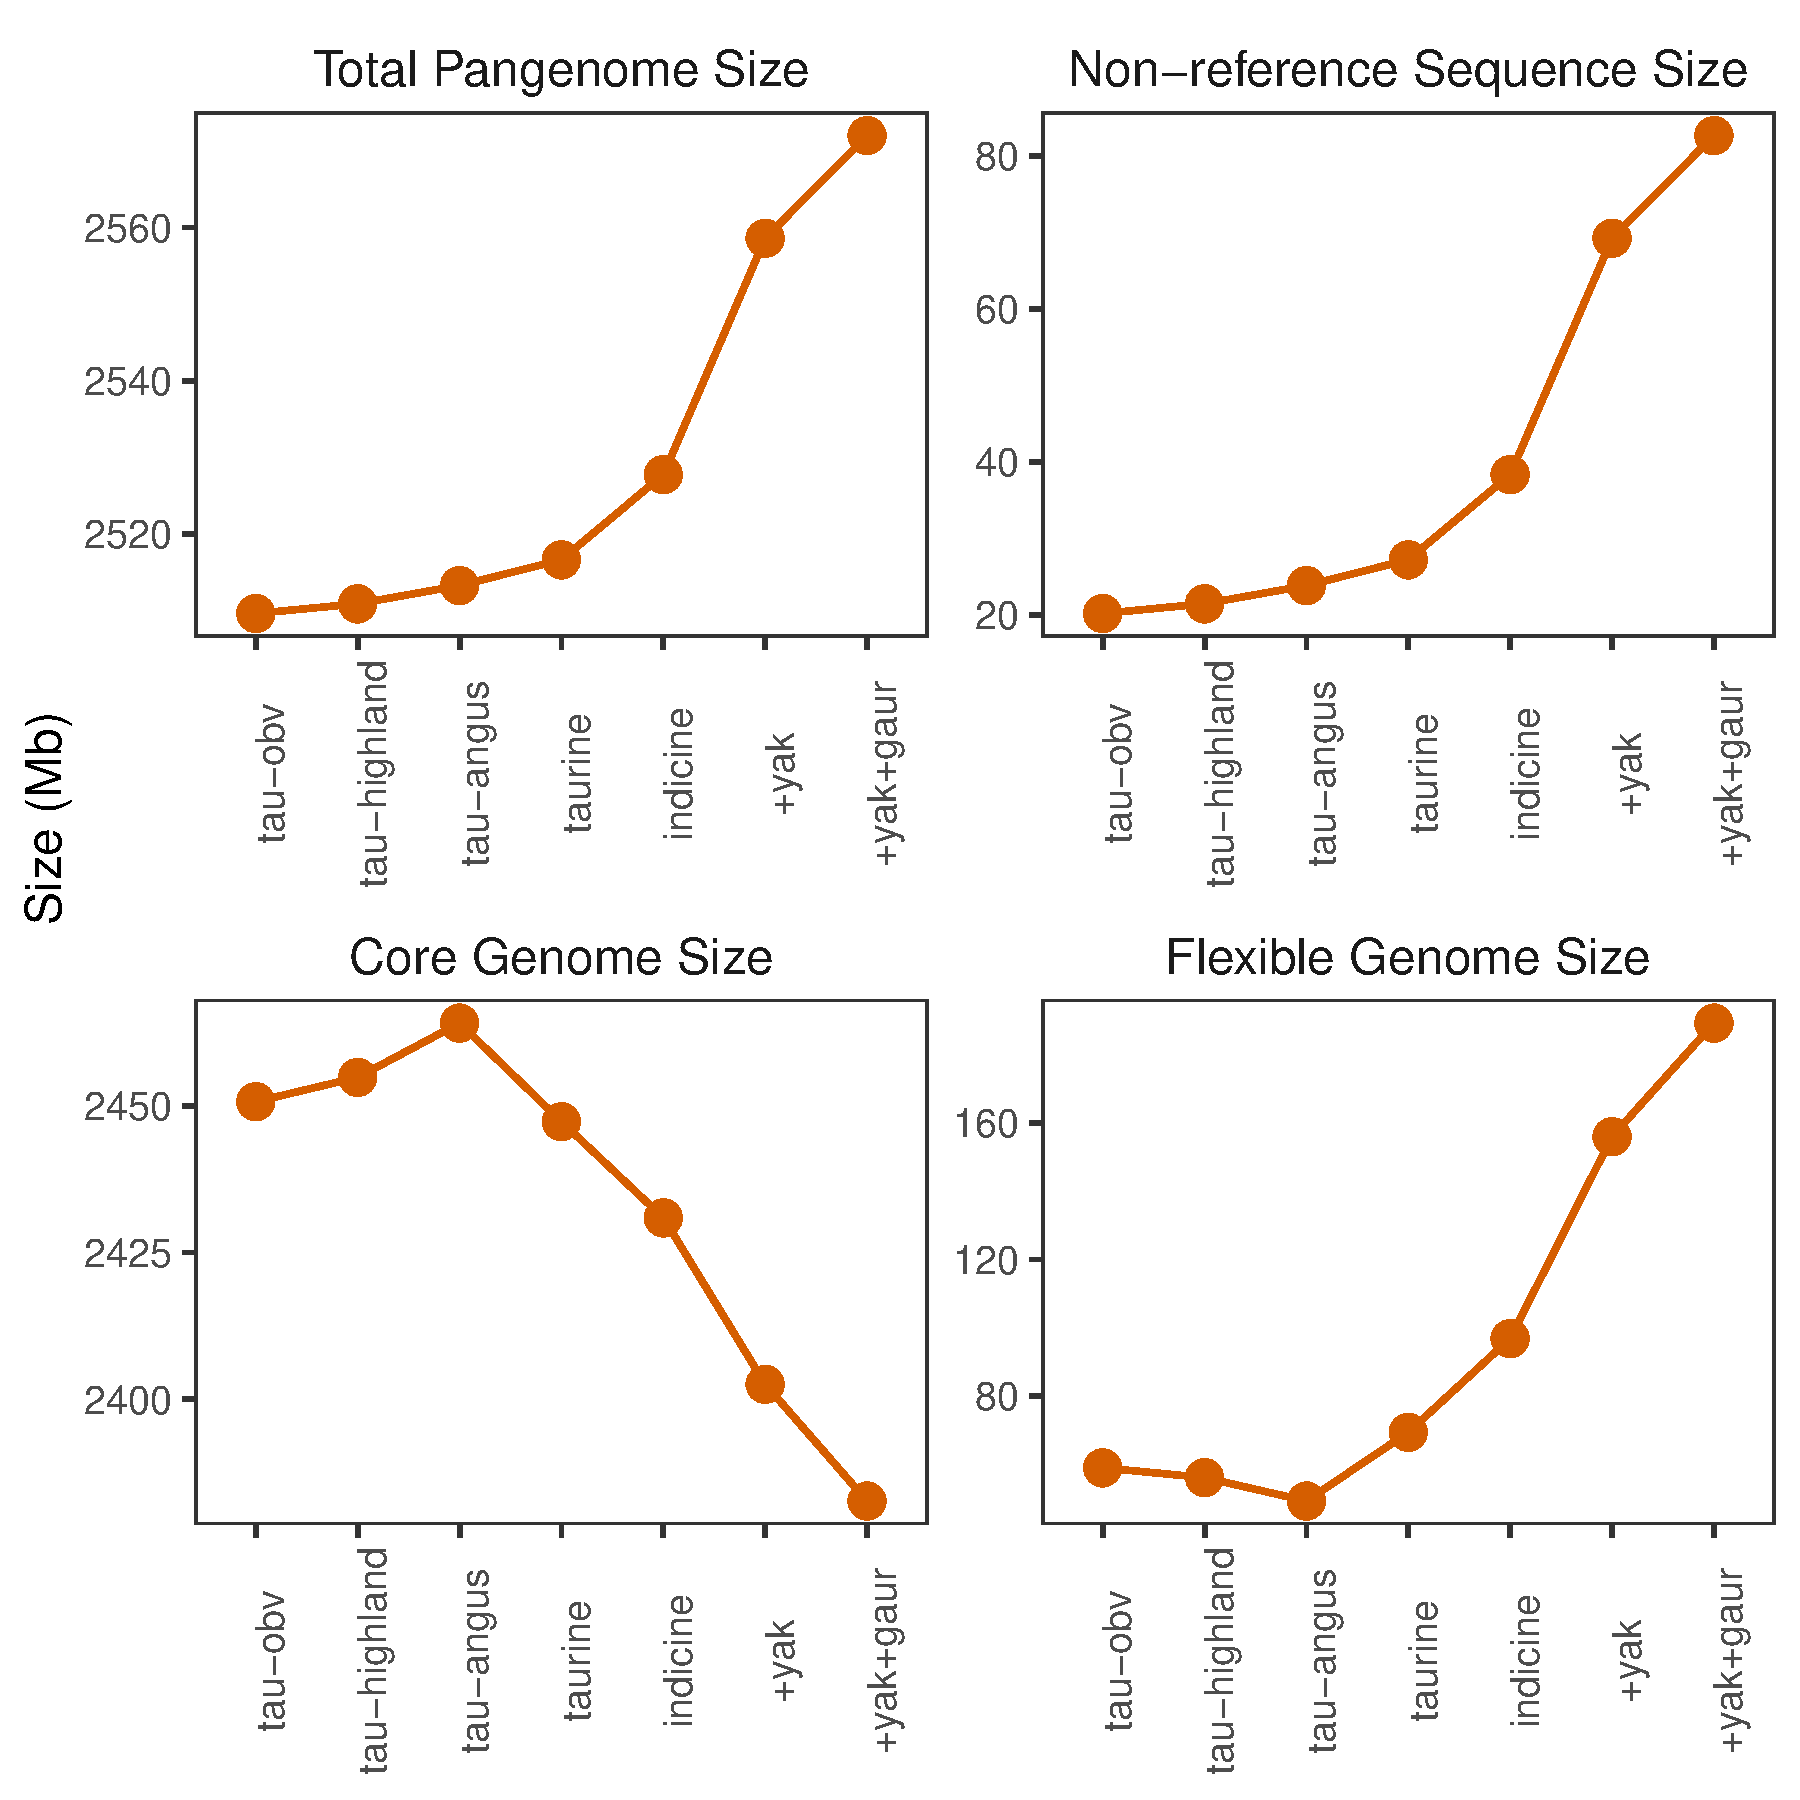
\includegraphics[width=0.9\textwidth]{discuss/fig51.pdf}
       \vspace{3mm}
       \caption[Pangenome graph profile as a more distant assembly added into the graphs]{\textbf{Pangenome graph profile as a more distant assembly added into the graphs.} \\
       \footnotesize{Pangenome graph was constructed as in Chapter 4 (4 taurine breeds, 1 indicine breed, 1 yak) with addition of the recently available gaur assembly. tau-$X$ denotes a graph with taurine assemblies but excluding breed $X$. Taurine indicates a graph with four taurine breeds. TauInd is a graph consisting of taurine + brahman genomes. +yak and +yak+gaur indicate the TauInd graph with an addition of yak and yak and gaur assembly, respectively. Non-reference sequence denote sequences not present in the reference assembly (ARS-UCD1.2). 
       The core and flexible genomes indicate sequences in pangenome shared in all and not in all breeds, respectively.
       }}
       \label{fig51:panchang}
\end{figure}


The construction of a comprehensive pangenome representing  global cattle diversity is the major aim of the Bovine Pangenome Consortium \citep{heaton2021reference}. Chapter 4 provides an initial framework to exploit these resources using a graph-based approach. The multi-assembly graph built from representative DNA sequences of cattle breeds might be starting point for the construction of a comprehensive bovine graphs. This is supported by Chapter 3 that global pangenome performed similarly as the population-specific pangenome. The sample selection should be carefully considered to maximize diversity (e.g. \citep{Ros-Freixedes2017,ranallo2021optimized}). The optimal sample selection that includes comprehensive and diverse breeds, including under-represented and wild and undomesticated relatives of the cattle, helps to characterize the complete pangenome content of Bovinae that will reveal the true extent of genetic diversity. Since generating reference-quality genome assemblies at the population scale is still prohibitively expensive, the strategy might be followed by enriching graphs with known small variations that are readily available from public databases. However, to avoid bias, this step is ideally done by iterative augmentation of variations discovered directly from the graphs. Further developments in the area of dynamic genome graphs are appealing that can iteratively update the graph as more genomes available or to subset a large graph into smaller graphs facilitating detailed inspection on the population of interest \citep{eizenga2020efficient}.

\subsection*{Towards highly informative graph genomes with the integration of functional genomics resources}

In addition to be comprehensive, graph genomes ideally should be informative. In the current implementation, graph genomes appear to be as static entity containing merely DNA sequence information. With added dimension than linear genomes, it opens the possibility to include additional information in the graph other than genome sequences itself, such as allele frequency, phenotype status of individuals the graph, or overlaying it with functional epi-genomic data. As a proof of concept, in Chapter 4, an extension of node labels of minigraph to track sample information is useful to characterize the origin of the non-reference sequences. For this purpose, strategy that can compactly store metadata information from large number of samples in the graphs needs to be explored e.g. \citet{siren2020haplotype}. 

Recent studies have examined the possibility of building more informative pangenome graphs. \citet{Sibbesen2021} performed pan-transcriptome study by adding splice information into a pangenome graph that outperformed the state-of-the-art RNA-seq mapper in the analysis involving allele-specific expression. \citet{Hokin2020} added genotype information and disease status of samples, enabling an association study directly from genotype graphs (termed as \emph{Pangenome Wide Association Study}). They found regions harboring complex variations the graph significantly associated with schizophrenia missed with a traditional GWAS. On the same line, \citet{kaye2021genome} proposed a Genome Atlas as an informative pangenome representation that graph nodes’ are labelled with a unique ID associated with rich functional metadata. The connections between nodes are not limited by sequence proximity, e.g., nodes could also be linked because of sharing annotation, which can be flexibly tuned. 

In this way, pangenome graphs can be used for integrated systems biology analysis with multiple genomics and epi-genomics data which might lead into broader understanding of the biological processes. This approach is readily feasible in livestock genomics with a vast array of functional omics data readily generated by genomic consortium such as FAANG \citep{clark2020faang}. Overall, these graph reference resources will be highly valuable for livestock community to catalogue the global cattle diversity in order to perform comprehensive comparative genomics or even to identify beneficial alleles relevant for the future environmental changes.  

\section{Challenges the construction of comprehensive pangenome graphs}

\subsection*{Importance of the genome assembly quality on the reliability of the graph-based analysis}

The quality of the assemblies being integrated into the graphs is important. Chapter 2 showed that in the regions with unresolved segmental duplications, the graph computation time increased substantially, indicating that the incomplete or the miss-assembly could spuriously increase the graph complexity. Additionally, some of the structural variations identified from graphs in Chapter 4 cannot be validated, which might also be due to miss-assembly. 
In this regard, long-read validation as implemented in Chapter 4 might be applicable to detect potential miss-assemblies from genomes integrated into graphs. 


With the minigraph approach, one assembly is used as the backbone of the graph and the pangenome is iteratively built by augmenting other genomes to this backbone. Therefore, the quality of assembly chosen as a backbone is critical for accurate and complete pangenome representation, especially to retrieve the real variable sequences diverged across animals rather than technical artifacts due to the incomplete assembly. Chapter 4 demonstrated that the use of Highland or OBV assembly as a backbone leads to a larger pangenome size with smaller amount of detected non-reference sequences (Figure \ref{fig52:backeff}). This finding possibly suggests that these two assemblies are more complete than other assemblies which aligns with previous claims \citep{rice2020continuous}. Interestingly, the effect of the assembly completeness is even more pronounced than the genetic distance of the backbone, which again emphasizing  the significance of high-quality assembly for the pangenome.  

\begin{figure}[!htb]
   \centering
   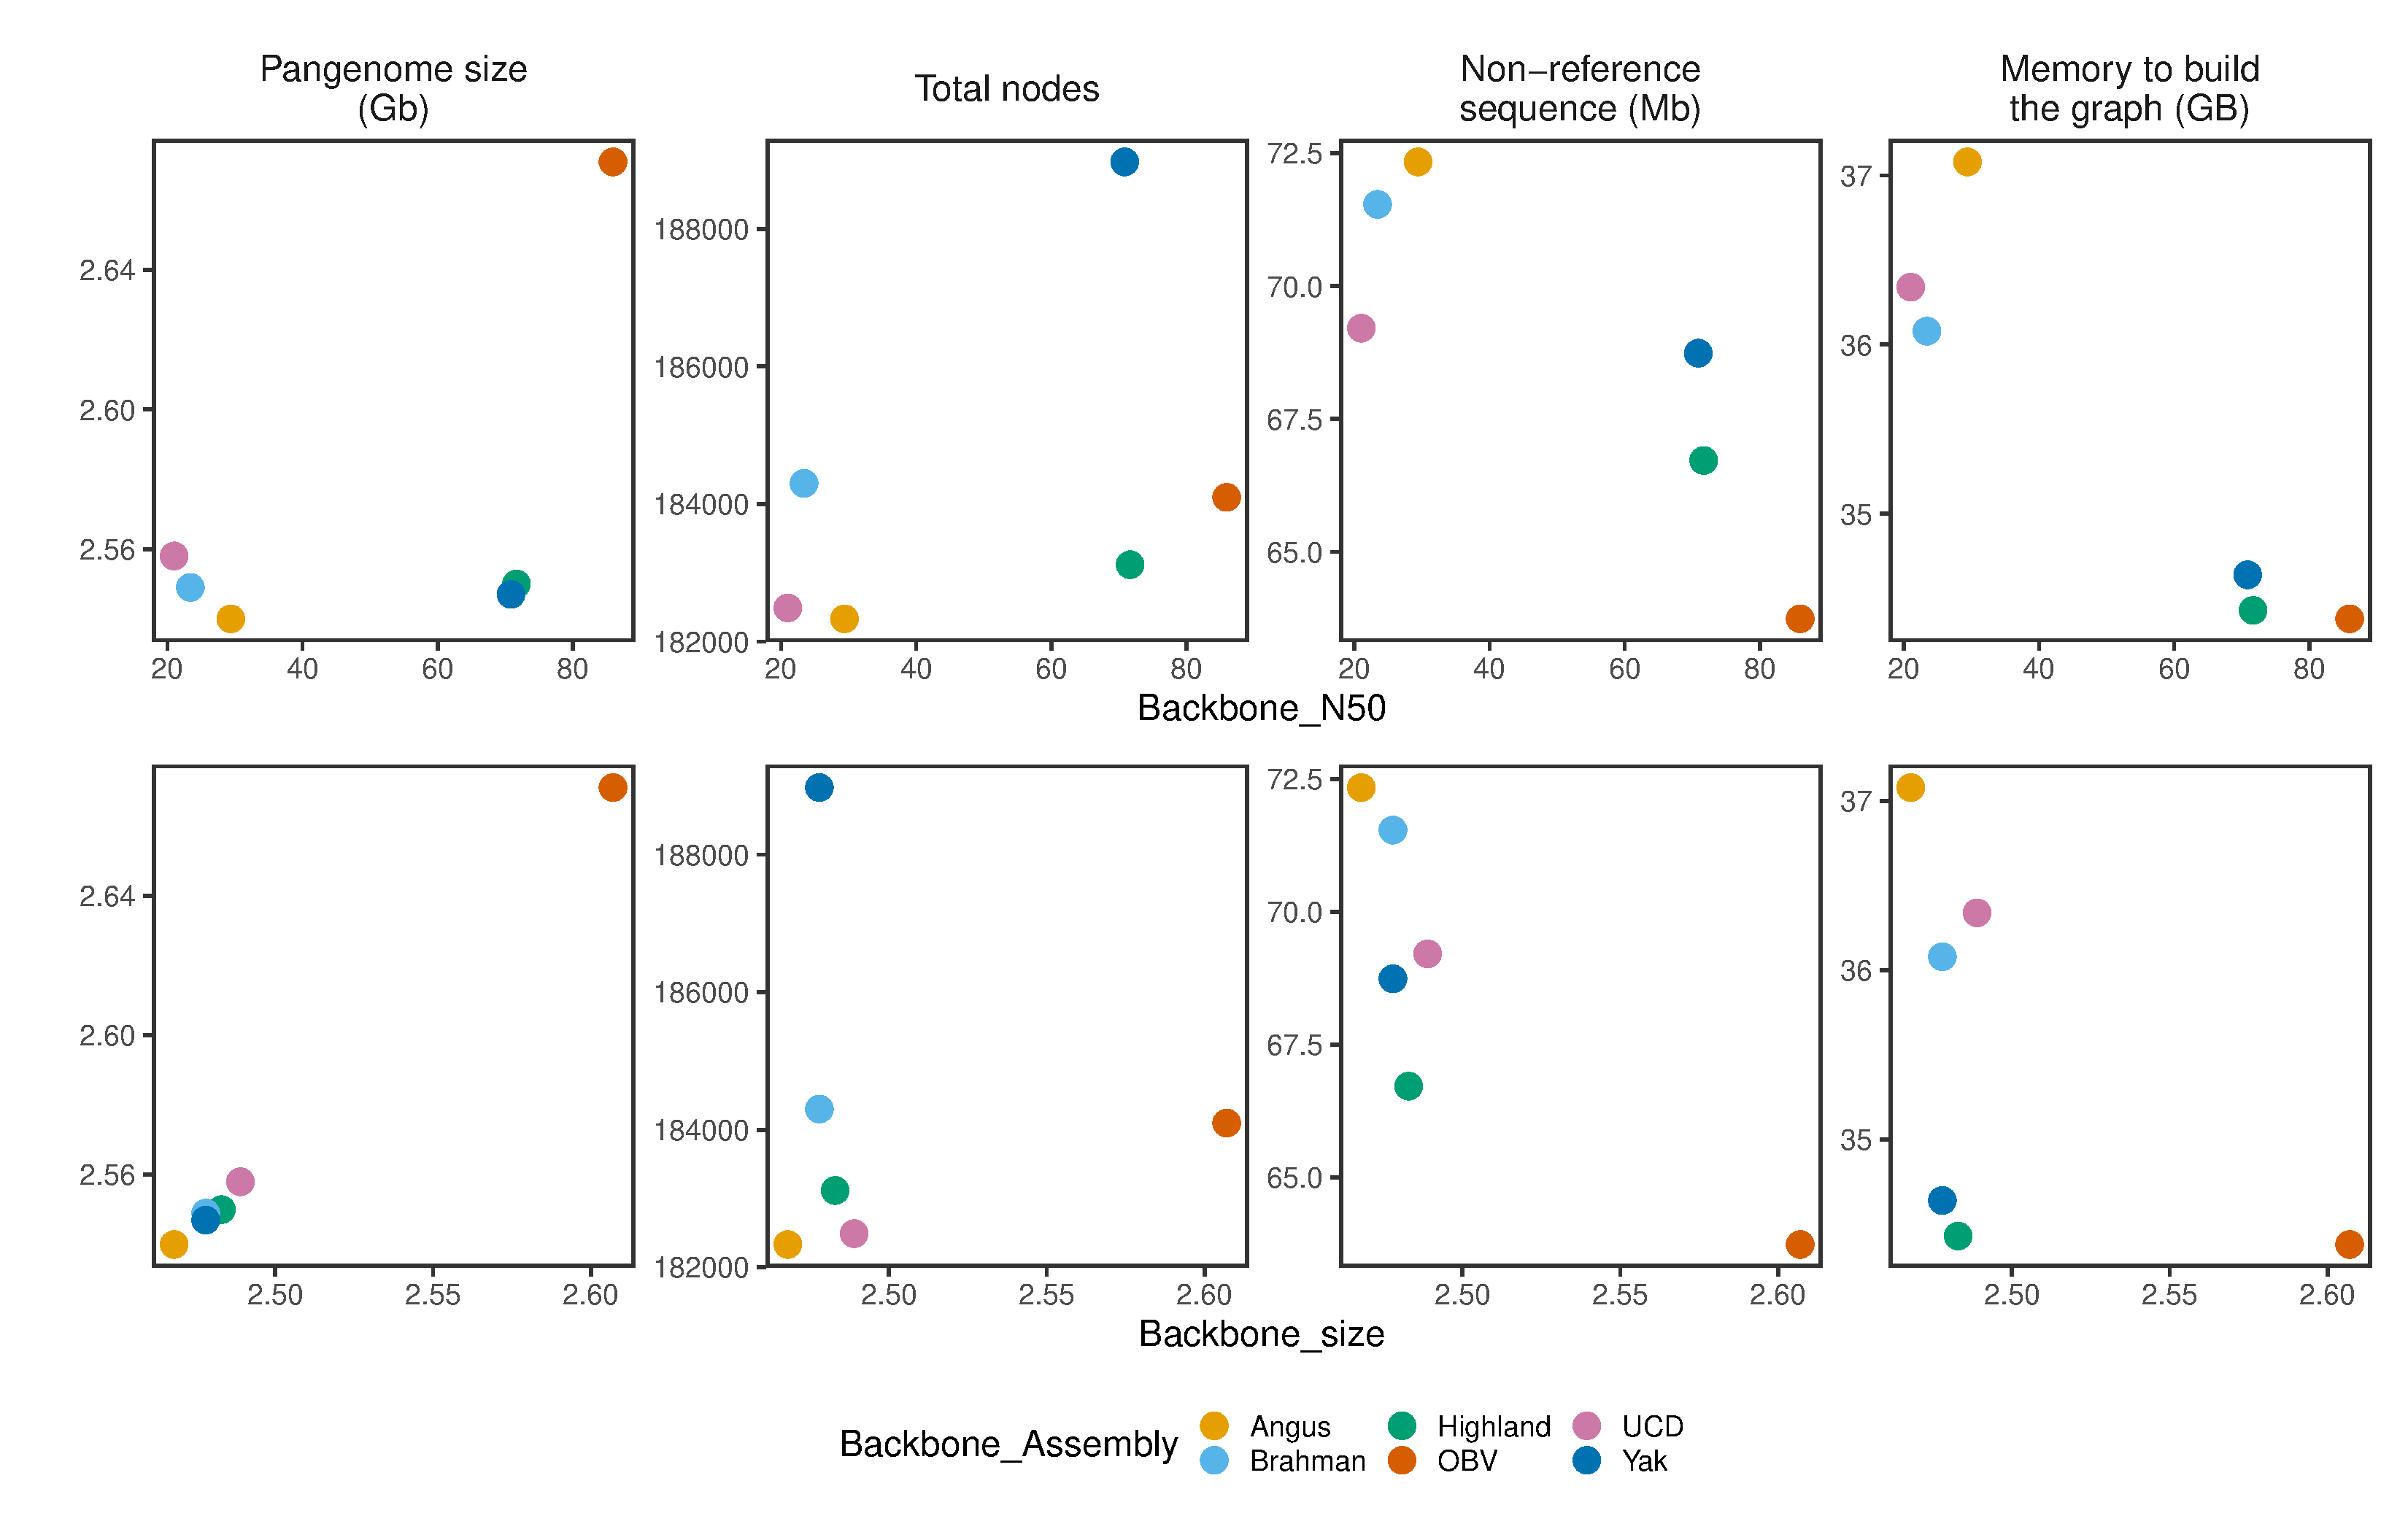
\includegraphics[width=\textwidth]{discuss/fig52.pdf}
       \vspace{1mm}
       \caption[Correlation between the backbone assembly size and quality with the profile of the pangenome graph]{\textbf{Correlation between the backbone assembly size and quality with the profile of the pangenome graph} \\
       \footnotesize{A colored dot represents the backbone assembly from which that the graph was built from. 
        N50 represents assembly contiguity with a higher number reflects a more contiguous assembly. 
       }}
       \label{fig52:backeff}
\end{figure}



Additionally, the pangenome will benefit from the use of resolved-haplotypes assemblies. The mapping algorithm in \emph{vg} (Chapter 3) utilized the phasing information to prioritize read alignment conforming to the haplotypes that can reduce ambiguous mapping. Moreover, haplotypes switches in collapsed assemblies might limit the interpretation of long-range information encoded in the paths. The value of haplotype-resolved assembly is recently shown in human pangenome graphs. Phasing information helps to infer the genotypes of low-coverage regions facilitating imputation-like strategy performed directly from the graphs \citep{ebler2020pangenome,ebert2021haplotype}. 

Technological advancements in long-read sequences particularly with the development of the highly-accurate circular consensus sequencing (HiFi) facilitates a cost effective production of high-quality genome assemblies to generate highly accurate pangenomes.  The multi-assembly graph constructed in Chapter 4 integrated the first Original Braunvieh assembly generated using HiFi reads. There were 104-116 Mb sequences from Original Braunvieh assembly not included in the graphs when other cattle assemblies used as a backbone. These sequences are primarily composed of DNA satellites, suggesting that the highly accurate long-reads used to construct the Original Braunvieh assembly enable a better assembly of so far difficult-to-assemble regions in the cattle genome, such as telomeric and centromeric sequences. Moreover, analyses in this thesis were restricted to the autosomal regions, due to lower quality of X, Y chromosomes, and unplaced contigs. Therefore, the high quality and complete assembly resolving complex regions (highly polymorphic or repeat regions) and sex chromosomes may serve as the backbone of the graphs \citep{logsdon2021structure,miga2020telomere} for a more accurate and complete pangenome.  

\subsection*{Scalable approaches for building comprehensive pangenome graphs across hundreds of assemblies }

Beyond generating assemblies, scalable approaches that can efficiently construct and characterize pangenome across a large number of assemblies are needed. Although the pangenome graph built using the minigraph approach as applied in the Chapter 4 is computationally efficient, the simplified graph it produces might not be ideal to represent the complete variations in the pangenome (Table \ref{tab52:mtc}). Thus, to exploit the full potential of the pangenome, full graph models that can account all haplotypes of the individuals in the population and including their sites of variations, are favored. Development a more comprehensive genome graph such as pggb or cactus pipeline is promising, that can perform reference-free multi-genome alignment to generate a full graph containing complete variations. Moreover, the resulting graphs will not be biased by not constraining it into a single genome as a backbone. Utilizing the full graph models as in pggb or cactus pipeline results in a detection of more variable genome and non-reference sequences (Table \ref{tab52:mtc}). However, it is still computationally intensive for a whole-genome scale graph. Moreover, the overall graph structure is a more complex with considerably more nodes of smaller size (Table \ref{tab52:mtc}). Additionally, without anchor genome the complex and highly repetitive genomic regions tend to form highly tangled regions in the graphs which are difficult to interpret \citep{lei2021plant}. Therefore, deep analysis assessing the tradeoff of various graph implementations are required. In fact, this is still in the area of a very active research, where it is likely that the strategy optimized by the Human Pangenome Reference Consortium (HPRC) to integrate 350 diverse human assemblies will set the standard in the field. 

\begin{table}[!htb]
   \begin{center}
   \small
   \caption[Comparison of methods to build the multi-assembly graphs]{\textbf{Comparison of methods to build the multi-assembly graphs.} \\

   \footnotesize{Ref nodes refer to the node contained sequences from the ARS-UCD1.2 reference genome and non-ref nodes contained sequences from the other breeds but not in the reference assembly. Core nodes and flexible represent nodes with sequences shared in all breeds and not in all breeds, respectively. R-R, R-NR, NR-NR denote edges connecting ref-ref nodes, ref-non-ref nodes, and non-ref-non-ref nodes respectively.}
   
   
   }
   \begin{tabular}{|l|l|l|l|l|} 
   \hline
   \multicolumn{1}{|c|}{\textbf{Parameter}} & \multicolumn{1}{c|}{\textbf{Unit}} & \multicolumn{1}{c|}{\textbf{Minigraph pipeline}} & \multicolumn{1}{c|}{\textbf{pggb pipeline}} & \multicolumn{1}{c|}{\textbf{Cactus pipeline}}  \\ 
   \hline
   Average memory                            & Mb                                 & 1,717                                            & 12,447                                      & 11,592                                         \\ 
   \hline
   Runtime                                   & seconds                            & 166.9                                            & 26,034                                      & 39,560                                         \\ 
   \hline
   All nodes                                 & n                                  & 1,136                                            & 804,723                                     & 843,177                                        \\ 
   \hline
   Total length                              & bp                                 & 42,671,567                                       & 43,495,189                                  & 43,583,632                                     \\ 
   \hline
   Average Node length                       & bp                                 & 37562                                            & 54                                          & 51                                             \\ 
   \hline
   Reference nodes                           & n                                  & 770                                              & 534,993                                     & 545,952                                        \\ 
   \hline
   Total length ref nodes                    & bp                                 & 42,350,435                                       & 42,316,615                                  & 42,350,435                                     \\ 
   \hline
   Non-reference nodes                       & n                                  & 366                                              & 269,730                                     & 297,225                                        \\ 
   \hline
   Total length non-ref nodes                & bp                                 & 321,132                                          & 1,178,574                                   & 1,233,197                                      \\ 
   \hline
   Total edges                               & n                                  & 1,630                                            & 1,384,318                                   & 1,142,667                                      \\ 
   \hline
   R-R edges                                 & n                                  & 904                                              & 706,505                                     & 570,277                                        \\ 
   \hline
   R-NR edges                                & n                                  & 705                                              & 631,949                                     & 524,483                                        \\ 
   \hline
   NR-NR edges                               & n                                  & 21                                               & 45,864                                      & 47,907                                         \\ 
   \hline
   Node to Edge Ratio                        & ratio                              & 1.43                                             & 1.72                                        & 1.35                                           \\ 
   \hline
   Core nodes                                & n                                  & 441                                              & 270,044                                     & 274,134                                        \\ 
   \hline
   Core length                               & bp                                 & 42,071,986                                       & 41,546,904                                  & 41,577,514                                     \\ 
   \hline
   Flexible nodes                            & n                                  & 695                                              & 534,679                                     & 569,043                                        \\ 
   \hline
   Flexible length                           & bp                                 & 59,9581                                          & 1,948,285                                   & 2,006,118                                      \\ 
   \hline
   Core proportion                           & \%                                 & 98.59\%                                          & 95.52\%                                     & 95.39\%                                        \\ 
   \hline
   Flexible proportion                       & \%                                 & 1.41\%                                           & 4.48\%                                      & 4.60\%                                         \\
   \hline
   \end{tabular}
   \label{tab52:mtc}
   \end{center}
   \footnotesize{$^*$ The multi-assembly graph was built from chromosome 25 of 4 taurine assemblies (Hereford, Angus, Highland, Original Braunvieh) and 1 indicine (Brahman) assembly. The minigraph pipeline was implemented as in the Chapter 4. The pggb pipeline was run with the recommended parameters (\texttt{-s 100000 -p 90 -n 10}, \url{https://github.com/pangenome/pggb}) and the cactus pipeline was based on the suggested within-species pangenome pipeline (\url{https://github.com/ComparativeGenomicsToolkit/cactus}). Both pggb and cactus pipeline implement a full graph model that includes complete variations, meanwhile minigraph only considers variations longer than 50 bp. \\
   }
\end{table}

\subsection*{Stable ecosystems and adoption of graph genomes in the genomic community}

In addition to strategy for building the graph, a stable ecosystem to efficiently store, modify, and handle graph for routine genomic analysis is not yet ready. Many analyses presented in this thesis were not fully graph-based that depends on the graph’s transformation into a linear coordinate that compatible with downstream tools that are still not yet graph-based. For example, genotyping on Chapter 3 was based graphs’ projection back to the reference sequence path to make it suitable with linear-genome-based variant calling tools. Thus, the reported improvement might actually be higher that can undermine the full potential of the graphs. Moreover, there are currently multiple fragmented graph implementations for limited use cases with poor interoperability among tools that might hamper the development of graph-based genomics. For example, due to differing in the specifications, graph structure from minigraph (Chapter 4) is not compatible with extensive graph operations already implemented in vg (Chapter 3). As the graph genome ecosystem become more mature, the genomic community may reach agreements on a single adopted standard that ensure long-term stability, which might mirror earlier tools development for a linear genome (e.g. \emph{BAM}, \emph{VCF}) \citep{bonfield2021htslib}. A wider adoption of graph-based analysis will naturally foster the development of efficient tools to process these new richer reference structures (e.g. \citep{qiu2021constructing,schulz2020detecting}). 


However, the genomics community might be reluctant to transition to graph-based approaches that might result in slower adoption of the methods. This direction will require a new paradigm and efforts  to adjust downstream tools that rely on a linear representation of the genome. Additionally, instead of a ready-to-use linear genome, graph genomes need a more involved construction process (see Chapter 3 Methods). However, this thesis clearly showed that the increase in the analysis complexity is outweighed by novel intriguing insights and graph approach is the way to go to integrate an ever increasing genomic resources. To attract the appeal of the graph genomes for the livestock community, it is highly desirable to have a robust graph-genome-based visualization for interactive explorations of the graph structure (e.g., coloring paths according to breeds that might help pinpoint segments differentiating between lineages). However, implementations that can accommodate across zoom levels and finer details are still open problems \citep{yokoyama2019momi,beyer2019sequence,eizenga2020pangenome}. In the short term, many proposed using graph approaches as intermediate steps hidden from the user, where the analysis performed on the graphs but the output projected back to the linear space. Thus, graphs will supplement rather than completely replace linear genomes \citep{kim2019graph,grytten2020assessing,li2020design,siren2020genotyping}. 

\newpage

\fancyhead[C]{OUTLOOK}
\section*{\LARGE{Outlook}}
\phantomsection
\addcontentsline{toc}{chapter}{Outlook}
\thispagestyle{plain}
This thesis presents the first step of the transition from linear to graph-based reference structure in cattle genomics. Pangenome graphs provide accurate, unbiased and complete catalogue of sequence variations of a species, such as sequence variations missed in routine genomic analysis because of the incomplete a single reference genome. The graph-based approaches implemented in this thesis could provide a starting point for many analyses that have not been possible so far (and less accurate) using the linear sequence, particularly for diverged sequences that are prone to the reference bias. Importantly, this thesis provides a computational framework to integrate and exploit an ever increasing genomic resources (including genome assemblies and their site of variations) that is relevant for genomic initiatives to catalogue the complete species diversity such as the Bovine Pangenome Consortium. Comprehensive comparative genomic analysis on the pangenome graph might help identify genomic features that are conserved across species or diverged that might underlying the adaptive traits, domestication, or evolution of livestock species which can then be exploited to accelerate genetic progress \citep{foissac2019multi,clark2020faang}. Finally, with continuing progress in long-read technology, the future of genomic might start by comparing an individual assembly with a collection of genomes from  a population (pan-genomes), rather than aligning sequencing data into a single genome (e.g. \citep{ebert2021haplotype}) which makes the concept of a single reference becomes obsolete.

Some areas in livestock genomics with potential applications of the genome graphs are discussed as below


\subsection*{Revisiting unbiased genomic analyses using genome graphs}

Genome graph approaches provide an immediate application to revisit genomic analyses that suffer from reference bias, such as Allele Specific Expression (ASE), which attempts to detect gene expression imbalance between paternal and maternal-derived alleles \citep{castel2020vast}. ASE has been known to be pervasive in cattle genome \citep{chamberlain2015extensive} and affects complex traits in livestock such as meat quality \citep{guillocheau2019survey,bruscadin2021muscle}. Current ASE detection method is primarily based on the RNA-sequencing mapping to a linear genome which is prone to reference allele bias. To overcome this issue, reference sequences are commonly modified to match the alleles from the transcriptome \citep{salavati2019elimination}. However, this strategy is imperfect as it needs two rounds of read mapping, limit alterations to SNPs, and can still underestimate the overall expression levels \citep{van2015wasp}. Genome graphs can represent both paternal and maternal alleles in a coherent structure that can mitigate this issue. Recently, the split-read mapping capability has been integrated in the \emph{vg toolkit} \citep{Sibbesen2021} that facilitate direct mapping of transcriptome data into the graphs. Therefore, it is appealing to revisit a more accurate ASE analysis in livestock using the graph genome approach. 

\subsection*{Comprehensive variations from pangenome might explain the missing heritability and improve genomic predictions}

So far, the catalogues of genetic variations cannot capture the full heritability of traits, widely known as missing heritability \citep{maher2008personal}. For example, a large meta-analysis on stature in cattle identified 163 lead variants, but these variants only explain about 13.8\% of the heritability of stature \citep{bouwman2018meta}. There were some proposals explaining the sources of heritability, such as the contribution of rarer variants \citep{gonzalez2015rare} that can be recovered when considering more comprehensive whole-genome variations \citep{wainschtein2019recovery}. However, complex structural variations and sequences not present in the reference genome which are not routinely assessed might 
a play role in explaining the heritability \citep{genin2020missing,theunissen2020structural}. The effect of large variations can be completely missed, which undermine its contribution to the genetic of traits. 

Multiple studies in humans \citep{eggertsson2019graphtyper2,chen2019paragraph,hickey2020genotyping} have attempted to integrate accurate and sequence-resolved structural variations from accurate representative long reads data into graphs, which can be then accurately genotyped using short-read data. Thus, it is appealing to revisit the genotyping of the vast amount of readily available of livestock short-read re-sequencing data using pangenome graph, which will provide a more comprehensive and accurate view of the structural changes in the genome. The genotype from complete variations of the population-scale pangenome can be used for robust genetic studies that might uncover some part of the missing heritability.

Genome-wide variants are frequently used to predict the animal’s phenotype, known as genomic prediction. It often relies only on SNPs or small variation markers from a single genome, which again prone to the ascertainment bias. 
There is already a recent effort to include more complete variations, such as structural variations in the genomic prediction. However, accounting this information only resulted in a small improvement than SNPs-based prediction \citep{el2018genomic,chen2021investigating}. This might be partly due to incomplete variations from resequencing data that pangenome graphs offer the ability to catalogues more accurate and unbiased variations from the population, such as in the genomic regions not present in a single reference. These diverged sequences might play a major role that give the breed its superior characteristics \citep{Hu2020}. Including more complete information may improve the accuracy breeding value predictions that leads to additional genetic gain. Additionally, graph genomes might be used to integrate diverse functional omics data for prioritizing variants used in genomic prediction. \citet{macleod2016exploiting} showed that stratification of variants with functional omics data improves prediction accuracy than treating all variants equally. 


\subsection*{Sequence variants in the pangenome might be causative for agriculturally important traits}

Most of the genomic analyses in livestock rely on the genetic markers discovered from a single reference genome, which might not be sufficiently representative for breeds diverged from the reference animal. The QTL or GWAS mapping will not be able to detect variants derived from segments not present in the reference sequences. Additionally, the fine mapping of the causative variants is not possible or very challenging if the genomic region overlapped with the structural variants that are not part of the reference sequences. In fact, the contribution of large variations in genetic of complex traits are known to be substantial, such as \citep{chiang2017impact,chaisson2019multi} suggesting that large structural variations are more likely to be associated with GWAS signal and have larger impacts on gene expression. Multiple studies in plants and humans have shown that GWAS signals can missed due to the genomic regions absent from the reference  \citep{kehr2017diversity,gage2019multiple,song2020eight}. \citet{song2020eight} performed association studies using the presence and absence of pangenome segment (termed as \emph{PAV GWAS}) across \emph{Brassica} plant accession enabling identification of large insertions, not part of the reference sequences, as causal variants for agriculturally important traits, such as seed weight and flowering time. Moreover, pangenome analysis of more than 15000 Icelander found a common 766 bp insertions \citep{kehr2017diversity} are associated with decreased risk of myocardial infarctions, that the signals are stronger than the SNPs-based association. These series of examples are an interesting area for potential application of the pangenome to dissect the genetic complex traits, which have not been done in the livestock population. \citet{hayes20191000} noted that the rate of identification of causal mutations for complex traits have been very slow in cattle, which might be contributed by genomic segments not yet included and annotated in the existing linear reference genome. 


\subsection*{Resources to catalogue and preserve the genetic diversity}

Domestication and selection of livestock species resulted in a considerable reduction of the genetic diversity compared to the wild relatives (termed as \emph{the cost of domestication}) \citep{mchugo2019unlocking} . Selection for desirable genes might be accompanied by unintentional removal of beneficial variants related to diseases, parasites of heat resistance relevant to current environmental changes. Thus, even though it carries superior production traits, the selected breeds might be more susceptible to environmental stresses. For example, successful breeding for milk yield in dairy cattle are accompanied with undesired impacts of declining fertility \citep{pryce2004fertility} and there is a negative genetic correlation between milk yield and mastitis resistance \citep{cai2020distinguishing}. 

Targeting the wild-relatives (non-domesticated) breed in the pangenome might help to identify genetic diversity which has been lost due to domestication and breeding that might be favorable for the future environmental changes. Thus, pangenome analysis need to expand into wild relatives and understudied breeds (termed as a \emph{super-pangenome} \citep{khan2020super}), which still possess the complete gene pool. The pangenome might be uncover the lost alleles (e.g., disease resistance gene) that can be introgressed back to the modern breeds or used to guide the gene-editing. Of note, genome assemblies of the undomesticated Bovinae \citep{wu2018pervasive}, including Bison (\emph{Bison bison})  and Gaur (\emph{Bos gaurus}) have been made publicly available, providing an opportunity to enrich cattle pangenome that captures the complete genetic diversity of a species (Figure \ref{fig51:panchang}). Additionally, the trio binning assembly technique perform better in a more heterozygous hybrid cattle from a more diverged parents \citep{rice2020continuous,heaton2021reference}. This provides exciting opportunities to generate assemblies using the understudied or undomesticated cattle relatives as one of the parental that facilitate generation of diverse collections cattle assemblies, which are ideal starting materials for a comprehensive bovine pangenome. 

Moreover, advances in modern genetics enables the creation of numerous specialized cattle breeds \citep{signer2017population,upadhyay2019genomic}. While the overall yield might increase with these local breeds, there is a cost in declining diversity might result in the loss of alleles that might be relevant in the future. Pangenome could facilitate identification of a collection of unique haplotypes that can be prioritized for conservation efforts. Thus, pangenome information potentially could be used to tailor breeding systems for improving production efficiency while preserving biodiversity.



\singlespacing
\footnotesize

% uncomment so that references appear on the same page
% \let\Origclearpage\clearpage
% \let\clearpage\relax

\bibliographystyle{unsrtnat}
\bibliography{references/discuss_ref}
%\printbibliography[title=References]

% \let\clearpage\Origclearpage

\ifdefined\BuildingFromMainFile
\else
   \end{document}
\fi